\part{Experiments}

\chapter{Benchmark POMDPs}

UVOD DO PROBLEMU< PROC JSME JE VYRALI< KDE JSOU ULOZENE ATD

Problems taken over from \cite{Littman} have changed transitions from terminal states. In the former problems, the environment is restarted with uniform transition to non-terminal states. In our implementation, the transition from terminal states are defined as deterministic transition to themselves. 


Chybi mi poradne benchmark problemy pro MDP

\subsection{1D Grid}
Custom 1D grid problem with custom number of states with terminal states on both ends, 2 actions (left and right), 30\% noise, 1. penalty for each action and 10. reward for getting to the terminal state.

\begin{figure}[h]
\caption{A 1D Grid environment}
\centering
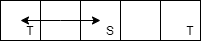
\includegraphics[scale=0.5]{1D_grid.png}
\end{figure}

\subsection{Pyramid}
Custom pyramid like problem designed specifically for Finite Horizon MDP solvers. Starting in the first stage with 1 state, the pyramid problem grows "upward", growing an additional state in each stage (first stage has 1 state, ..., n$^th$ stage has n states). The Pyramid MDP has 2 possible actions, moving down-left, or down-right. The user can optionally define terminal states. By default the terminal states are contained in the last stage.

\begin{figure}[h]
\caption{A Pyramid environment}
\centering
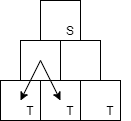
\includegraphics[scale=0.5]{Pyramid.png}
\end{figure}

\subsection{Mini Hallway \cite{Littman}}

Small navigation problem consisting out of 13 states. The environment is created from 3 rooms with 4 orientations and 4$^{th}$ terminal room denoted by a start, 9 observations (relative locations of surrounding walls) and 3 actions (forward, rotate left, rotate right.
The problem models mini hallway with robot whose task is to enter the room marked with the star for which the agent gets the reward +1. The transitions and observations are deterministic
\begin{figure}[h]
\caption{A Mini Hallway environment}
\centering
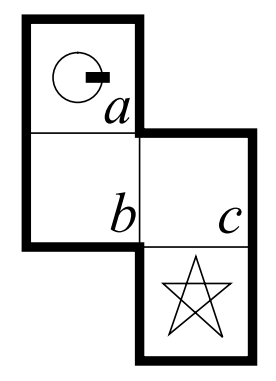
\includegraphics[scale=0.5]{MiniHallway.png}
\end{figure}

\subsection{Hallway \cite{Littman}}

Middle sized navigation problem consisting out of 60 states. The environment is created from 14 rooms with 4 orientations each and one room with 4 terminal states. Other than that, the model contains 21 observations (possible combinations of walls presence. star - terminal states and three numbered landmarks) and 5 actions (stay in place, move forward, turn right, turn left, turn around). Both transitions and observations are extremely noisy.

\begin{figure}[h]
\caption{A Hallway environment}
\centering
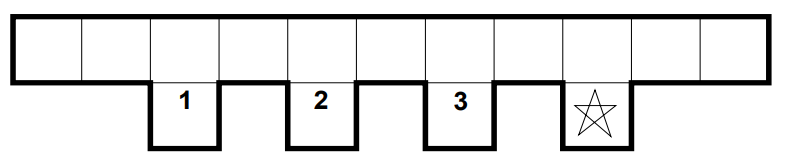
\includegraphics[scale=0.5]{hallway.png}
\end{figure}


\begin{table}[h!]
\centering
\begin{tabular}{||c c c c c c c||} 
 \hline
 Domain & |S| & |A| & |\Omega| & Observability & Transitions & Observations \\
 \hline\hline
 1D Grid & custom & 2 & 0 & Fully Observable & Stochastic & Null \\
 Pyramid & custom & 2 & 0 & Fully Observable & Stochastic & Null \\
 MiniHallway & 13 & 3 & 9 & Partially Observable & Deterministic & Deterministic \\
 Hallway & 60 & 5 & 21 & Partially Observable & Stochastic & Stochastic \\
 \hline
\end{tabular}
\caption{Table to test captions and labels}
\label{table:1}
\end{table}


Tag????